\documentclass[a4paper,11pt]{article}
\usepackage{amsmath}
\usepackage{amsfonts}
\usepackage{textcomp}
\usepackage{amssymb}
\usepackage{graphicx}
\usepackage{fancyhdr}
\usepackage[spanish]{babel}
\usepackage[utf8]{inputenc}
\usepackage{array}
\usepackage[usenames,dvipsnames,svgnames,table]{xcolor}
\usepackage{multirow}


\definecolor{niceblue}{RGB}{60,110,190}

\usepackage{vmargin}
\setpapersize{A4}
\setmarginsrb{2.5cm}{1.5cm}{2.5cm}{2.5cm}
{1cm}{0cm}%
{1cm}{1cm}

\begin{document}

\begin{tabular}{ >{\centering\arraybackslash}m{4cm} >{\arraybackslash}m{8cm}}
\fbox{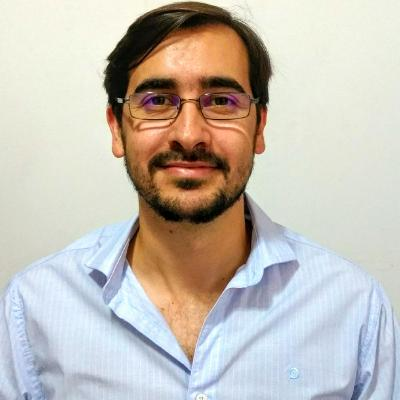
\includegraphics[width=25mm]{rodrigo}} & {\huge Dr. Rodrigo Baravalle}
\end{tabular}
\vspace{0.5cm}

\begin{small}
\begin{tabular}{ll}
\bf{\color{Gray}City} & Rosario, Argentina\\
\bf{\color{Gray}Date of Birth}  & 20 April 1985\\
\bf{\color{Gray}Place of Birth}  & Rosario, Santa Fe, Argentina\\
\bf{\color{Gray}Marital Status}  & Married\\
\bf{\color{Gray}E-Mail} &rbaravalle@gmail.com\\
\end{tabular}
\end{small}

\section*{\color{niceblue} \rule{2cm}{2.2pt} About}

\begin{small}
\noindent
I am currently on a research internship at iRobot, after finishing my postdoc.
I completed my PhD on March 2016 (Photo-realistic material modeling and simulation).
My foremost academic interests are Image Processing, Deep Learning, Computer Vision, Robotics and Computer Graphics. 
In addition, I am keen on reading about astronomy, physics, psychology and philosophy. Also, I eventually play chess.
\end{small}


\section*{\color{niceblue} \rule{2cm}{2.2pt} Education}

\begin{tabular}{lcp{12 cm}}
		\bf{2018} & & {\bf PostDoc} (Photo-realistic bone modeling and simulation). CONICET, Argentina. \\
		\bf{2016} & & {\bf PhD in Computer Science} (Photo-realistic material modeling and simulation). FCEIA - Universidad Nacional de Rosario. \\
		\bf{2010} & & {\bf Licenciateship in Computer Science}. FCEIA - Universidad Nacional de Rosario. Academic Average: 9.4 ``Distinguished''.\\
\end{tabular}

\section*{\color{niceblue} \rule{2cm}{2.2pt} Work Experience}

\begin{itemize}
\item {\bf Research Internship} at {\em iRobot}, Pasadena, USA. Image Processing and Deep Learning. April 2018 - Today.
\item {\bf Postdoc Fellowship}, at {\em CONICET}, Photo-realistic modeling of porous materials, machine learning for several applications. April 2016 - March 2018.
\item {\bf Research Internship} at {\em iRobot}, Pasadena, USA. Image Segmentation for robot vacuum cleaners. September 2015 - December 2015.
\item {\bf PhD Student}, at {\em CONICET, Universidad Nacional de Rosario}, Photo-realistic modeling of porous materials. April 2011 - March 2016.
\item {\bf Research Internship} at {\em E-MOTION, Inria}, Grenoble, France. 3D Reconstruction from a Time-of-Flight Camera. September 2010 - February 2011.
\end{itemize}

\newpage

\section*{\color{niceblue} \rule{2cm}{2.2pt} Skills }

\begin{itemize}
\item C++, C, Python, bash, Matlab.
\item git, SVN, Linux.
\item Tensorflow-lite, Keras.
\end{itemize}


\section*{\color{niceblue} \rule{2cm}{2.2pt} Recent Publications}

\subsection*{\color{niceblue} Journals}

\begin{itemize}
\item {\bf Real-time Dense Map Fusion for Stereo SLAM}. Taihú Pire, Rodrigo Baravalle, Ariel D'alessandro and Javier Civera. {\it Robotica}, 2018. In press.
\item {\bf Three Dimensional Multifractal Analysis of Trabecular Bone under Clinical Computed Tomography}. Rodrigo Baravalle, Félix Thomsen, Claudio Delrieux, Juan Carlos Gómez, Borko Stosic, Tatijana Stosic. In {\it Medical Physics}, {\bf 44}(12):6404-6412, December 2017. doi:10.1002/mp.12603.
\item {\bf Realistic Modeling of Porous Materials}. Rodrigo Baravalle, Leonardo Scandolo, Claudio Delrieux, Cristian García Bauza and Elmar Eisemann. In {\it Computer Animation \& Virtual Worlds}, 2016. doi:10.1002/cav.1719.
\item {\bf Procedural Bread Making}. Rodrigo Baravalle, Gustavo Patow and Claudio Delrieux. In {\it Computers \& Graphics}. {\bf 50}(2015):13-24. doi:10.1016/j.cag.2015.05.003.
\item {\bf Multifractal Characterisation and Classification of Bread Crumb Digital Images}. Rodrigo Baravalle, Claudio Delrieux and Juan Carlos Gómez. In {\it EURASIP Journal on Image and Video Processing}. {\bf 2015}:9. April 2015. doi:10.1186/s13640-015-0063-8.
\end{itemize}


\subsection*{\color{niceblue} Conferences}
\begin{itemize}
\item {\bf A Solution to Room-by-Room Coverage for Autonomous Cleaning Robots}. Alexander Kleiner, Rodrigo Baravalle, Andreas Kolling, Pablo Pilotti and Mario Munich. In {\it Proceedings of the International Conference on Intelligent Robots and Systems}, IROS. Vancouver, Canada. September 2017.
\end{itemize}

\subsection*{\color{niceblue} Technical Reports}
\begin{itemize}
\item {\bf 3D Mapping of Indoor Environments with a Time of Flight Camera}. Rodrigo Baravalle and Amaury N\`egre. E-MOTION (INRIA Grenoble Rh\^one-Alpes / LIG Laboratoire d'Informatique de Grenoble) Number: RT0406. Grenoble, France, February 2011.
\end{itemize}



\section*{\color{niceblue} \rule{2cm}{2.2pt} Courses Given}
\begin{itemize}
\item {\bf Introduction to Computer Graphics} at the Computer Science Department at UNR (Rosario, Argentina. November 2014).
\end{itemize}

\section*{\color{niceblue} \rule{2cm}{2.2pt} Teaching Experience}

Teacher assistant at the Computer Science Department at UNR (Rosario, Argentina) on different courses:
\begin{itemize}
\item Data Structures and Algorithms I. March - August 2012.
\item Computer Architectures. September 2012 - February 2013.
\end{itemize}

\section*{\color{niceblue} \rule{2cm}{2.2pt} Grade Thesis Advised}
\begin{itemize}
\item {\bf Dense 3D stereo reconstruction of SLAM Systems}. Ariel D'Alessandro. Co-Advisor. National University of Rosario, Argentina, {\it Finished on December 2017}. Grade: 10 (Ten).
\end{itemize}

\section*{\color{niceblue} \rule{2cm}{2.2pt} Grade Thesis Evaluator}
\begin{itemize}
\item {\bf Adversarial Neural Networks for weed recognition}. Universidad Nacional de Rosario, Argentina, February 2018.
\item {\bf Multi-class learning of sport videos with deep learning}. Martín Escarrá. Universidad Nacional de Rosario, Argentina, March 2016.
\end{itemize}

\section*{\color{niceblue} \rule{2cm}{2.2pt} Languages}

\begin{small}
\begin{description}
	\item[Spanish:] Native language.
	\item[English:] First Certificate In English (FCE) (Level B2), by University of Cambridge, ESOL. Certificate Number: 0026091410. February 2010.
	\item[French:] DELF B2 Certificate (Level B2), by Alliance Fran\c{c}aise. Certificate number: 054041-201311T-2234032. April 2014.
\end{description}
\end{small}

\section*{\color{niceblue} \rule{2cm}{2.2pt} References}

\begin{itemize}
	\item {\bf Dr. Alexander Kleiner}, PhD. President Artificial Intelligence \& Machine Learning at FaceMap LLC, USA.\\E-mail: alexander.kleiner@gmail.com. \\
	\item {\bf Dr. Claudio Delrieux}, PhD. Head of the Department of Electrical Engineering and Computers, Universidad Nacional del Sur, Argentina.\\E-mail: cad@uns.edu.ar\\
	\item {\bf Dr. Gustavo Patow}, PhD. Head of the Geometry and Graphics Group (GGG), Girona, Spain.\\E-mail: dagush@imae.udg.edu \\
\end{itemize}

\end{document}




